\documentclass{standalone}
\usepackage{tikz}
\usepackage{pgfplots}
\pgfplotsset{width=32cm,height=18cm,compat=1.3}
\pgfplotsset{every tick label/.append style={font=\Huge}}
\usepackage{filecontents}

\usetikzlibrary{patterns}

\definecolor{citrine}{rgb}{0.89, 0.82, 0.04}

\begin{document}
	\centering
		\vspace{1.5em}
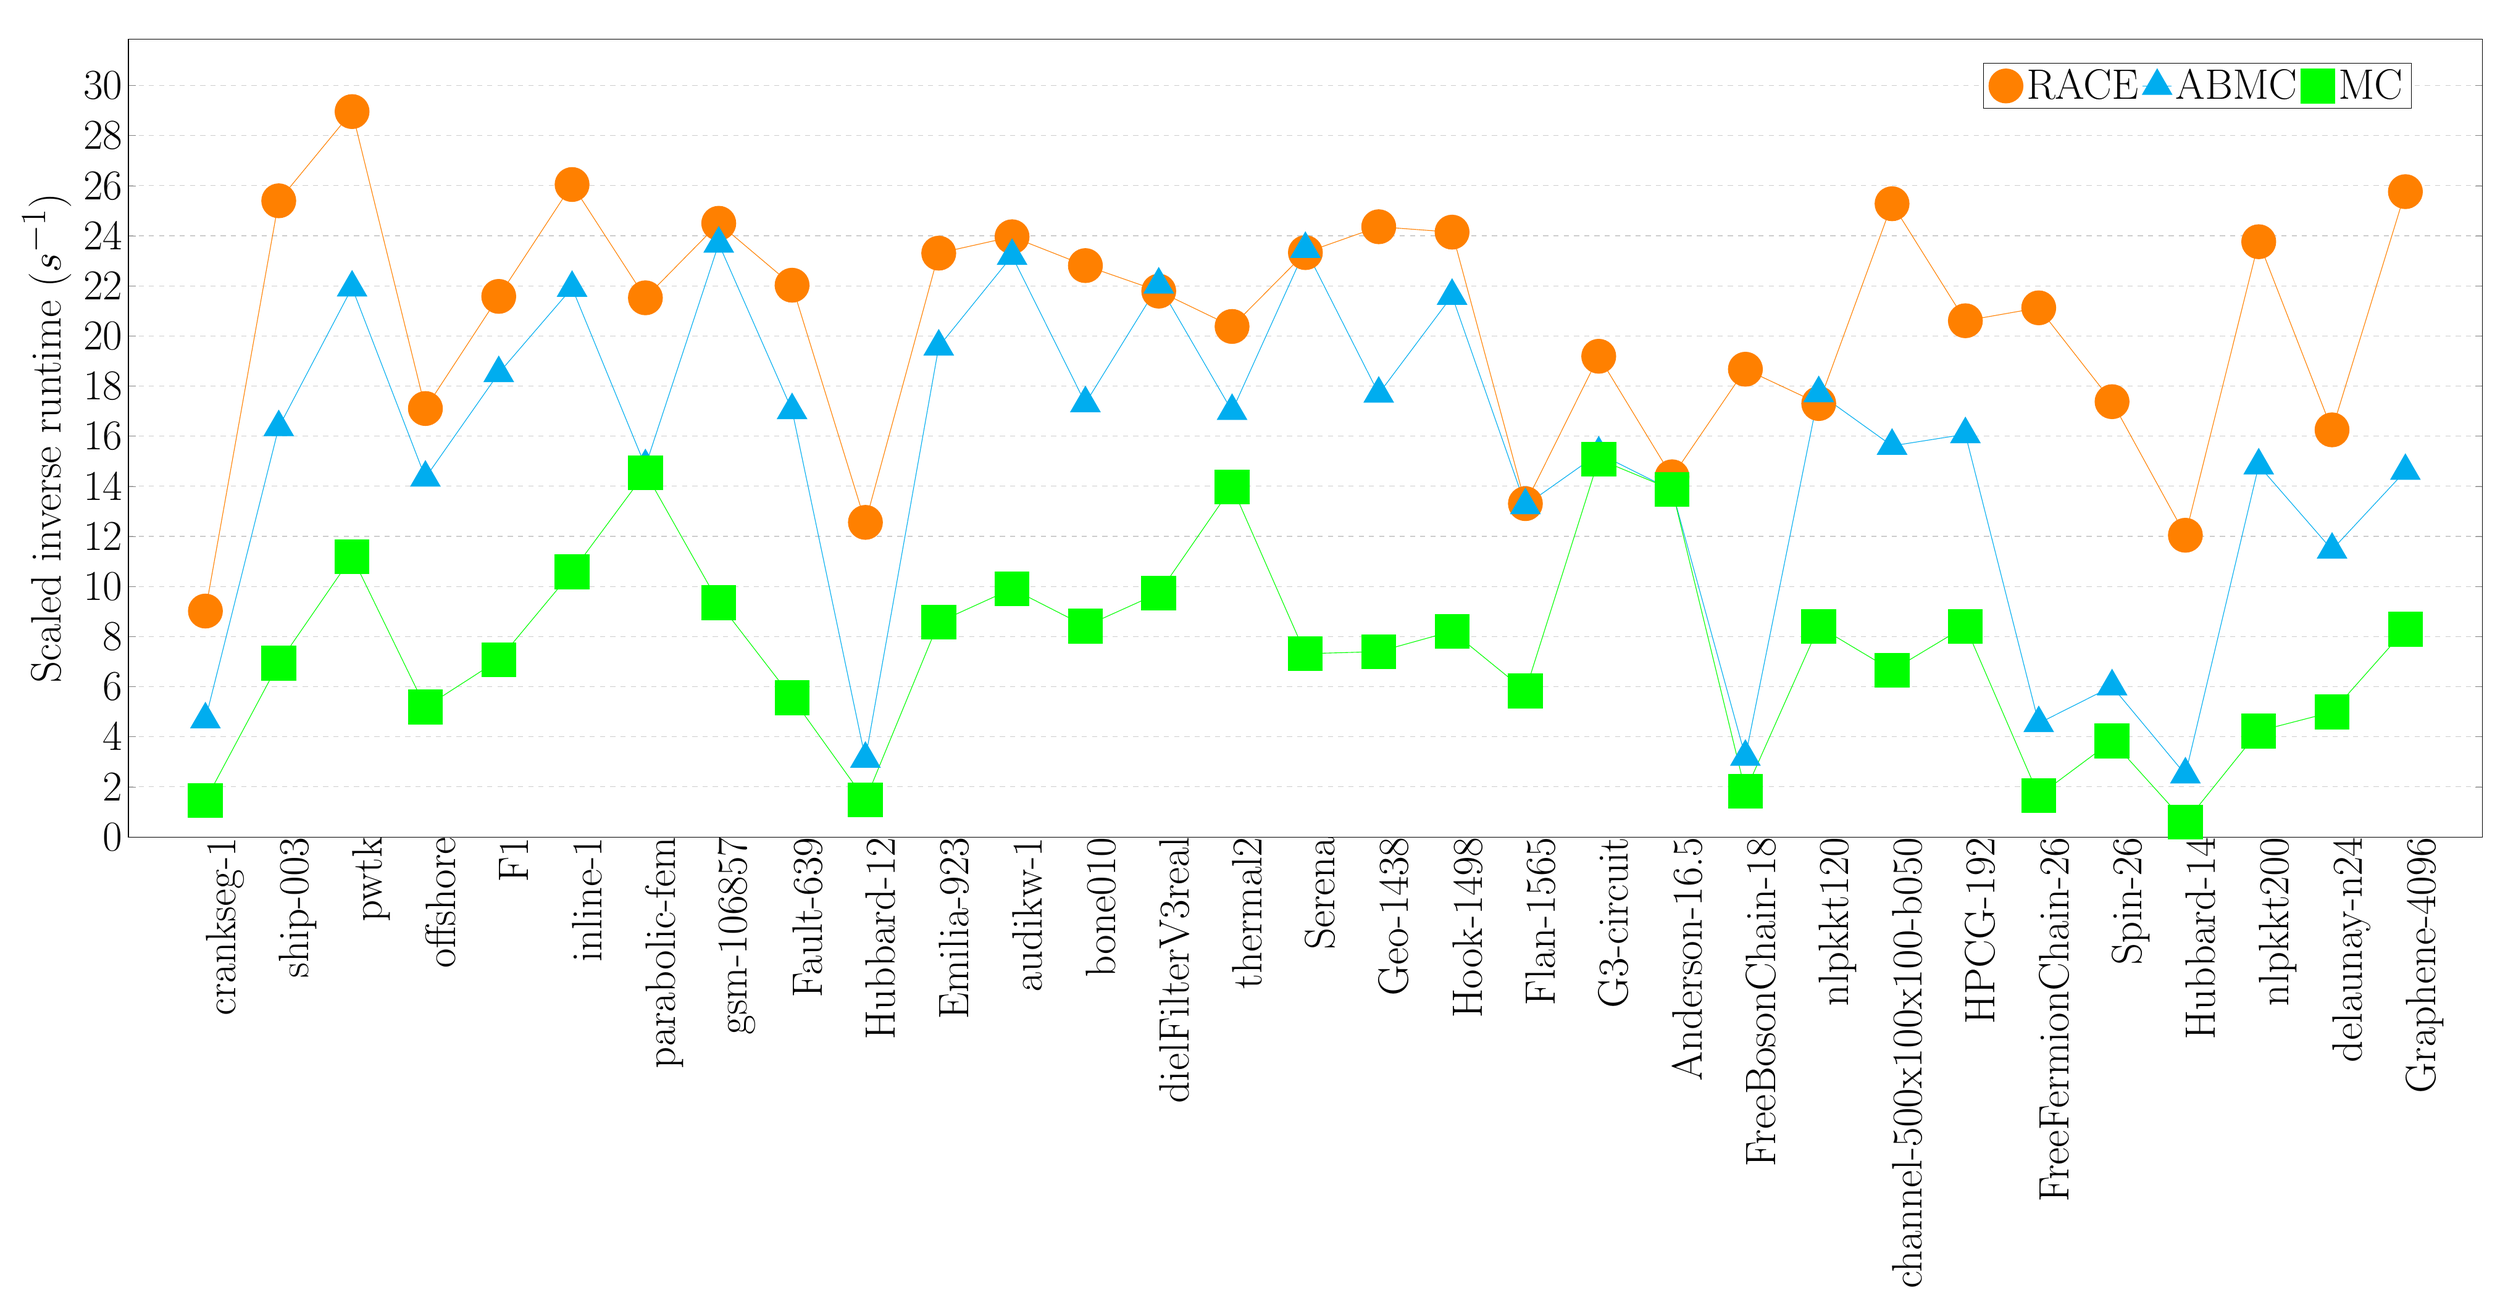
\begin{tikzpicture}
		%	\node at (13.25,15) {\LARGE{}};
			\begin{axis}[
		%	xmin=0.25, xmax=7.25,
			ymin=0, %ymax=3.25,
			xtick={1, 2, 3, 4, 5, 6, 7, 8, 9, 10, 11, 12, 13, 14, 15, 16, 17, 18, 19, 20, 21, 22, 23, 24, 25, 26, 27, 28, 29, 30, 31},
		%	ytick={0,0.5,1,1.5,2,2.5,3},
			xticklabels={crankseg-1, ship-003, pwtk, offshore, F1, inline-1, parabolic-fem, gsm-106857, Fault-639, Hubbard-12, Emilia-923, audikw-1, bone010, dielFilterV3real, thermal2, Serena, Geo-1438, Hook-1498, Flan-1565, G3-circuit, Anderson-16.5, FreeBosonChain-18, nlpkkt120, channel-500x100x100-b050, HPCG-192, FreeFermionChain-26, Spin-26, Hubbard-14, nlpkkt200, delaunay-n24, Graphene-4096},
			width  = 50cm,
			height = 18cm,
			major x tick style = transparent,
			%	minor ytick={1, 5, 10, 15, 20, 25, 30 ,35,40},
			grid = minor,	
			%add_bar_commands
			ymajorgrids = true,
			grid style={dashed, gray!40},
			ylabel = {\Huge{Scaled inverse runtime ($s^{-1}$)}},
		%	symbolic x coords={Graphene-2048-2048, Graphene-4096-4096, Spin-24-24-24},
			x tick label style={rotate=90, anchor=north east, inner sep=0mm, font={\Huge}},
			tick label style={font={\Huge}},
			scaled y ticks = false,
			enlarge x limits=0.035,
			legend cell align=left,
			legend style={font=\Huge},
			legend columns=-1,
			legend style={
				%at={(1,1.05)},
				%anchor=south east,
				%column sep=1ex,
				legend pos=north east
			},
			%spl_legend_code
			title= {\Huge\scalebox{1.5}{{}}}
			]

\addplot[ mark=*, mark size=10pt, mark options={orange}, draw=orange , y filter/.code={\pgfmathparse{\pgfmathresult*1000}\pgfmathresult}] plot coordinates{(1,.00901802450980392156) (2,.02539598932038834951) (3,.02895739611650485436) (4,.01710322135922330097) (5,.02157931960784313725) (6,.02604576700000000000) (7,.02152336476190476190) (8,.02449889306930693069) (9,.02202627327586206896) (10,.01255866938775510204) (11,.02330574690265486725) (12,.02396078333333333333) (13,.02280905142857142857) (14,.02178962549019607843) (15,.02037944851485148514) (16,.02332725714285714285) (17,.02435985673076923076) (18,.02414455961538461538) (19,.01330639027027027027) (20,.01918933523809523809) (21,.01437837642276422764) (22,.01867283009708737864) (23,.01730216696428571428) (24,.02527885436893203883) (25,.02060781333333333333) (26,.02112321265822784810) (27,.01737666261682242990) (28,.01204455620915032679) (29,.02376221747572815533) (30,.01625191359223300970) (31,.02576133069306930693)};
\addplot[ mark=triangle*, mark size=10pt, mark options={cyan}, draw=cyan , y filter/.code={\pgfmathparse{\pgfmathresult*1000}\pgfmathresult}] plot coordinates{(1,.00468924705882352941) (2,.01635329363636363636) (3,.02192804529914529914) (4,.01433925242718446601) (5,.01851341759259259259) (6,.02191773853211009174) (7,.01479597280000000000) (8,.02368184951456310679) (9,.01703387397260273972) (10,.00311718657718120805) (11,.01957295000000000000) (12,.02319240849056603773) (13,.01731059428571428571) (14,.02204990446428571428) (15,.01700272571428571428) (16,.02347179600000000000) (17,.01769161632653061224) (18,.02159944957983193277) (19,.01323878783068783068) (20,.01530750588235294117) (21,.01384084196428571428) (22,.00319763267326732673) (23,.01771228934426229508) (24,.01561314344262295081) (25,.01607515203252032520) (26,.00453882500000000000) (27,.00600935087719298245) (28,.00249264357976653696) (29,.01482769274193548387) (30,.01146475517241379310) (31,.01461067407407407407)};
\addplot[ mark=square*, mark size=10pt, mark options={green}, draw=green , y filter/.code={\pgfmathparse{\pgfmathresult*1000}\pgfmathresult}] plot coordinates{(1,.00145511496062992125) (2,.00693956637168141592) (3,.01119306776859504132) (4,.00518439333333333333) (5,.00706734240000000000) (6,.01058904653465346534) (7,.01454017902097902097) (8,.00935457727272727272) (9,.00555758282208588957) (10,.00147422775423728813) (11,.00857907278911564625) (12,.00990892121212121212) (13,.00841590123456790123) (14,.00973562222222222222) (15,.01397376544117647058) (16,.00731630707964601769) (17,.00739855220125786163) (18,.00821216267605633802) (19,.00582675036231884057) (20,.01507995785123966942) (21,.01386703587786259541) (22,.00182514595238095238) (23,.00839940151515151515) (24,.00665142733812949640) (25,.00840984632352941176) (26,.00165275477031802120) (27,.00383155426356589147) (28,.00058974275000000000) (29,.00422964701492537313) (30,.00498569493670886075) (31,.00829041448275862068)};
	%addplot cmd

	\legend{RACE, ABMC, MC}

	\end{axis}			
\end{tikzpicture}

\end{document}

